\chapter{Metodología}\label{cap4:Metodologia}

\section{Metodología}

\begin{figure}[H]
    \centering
       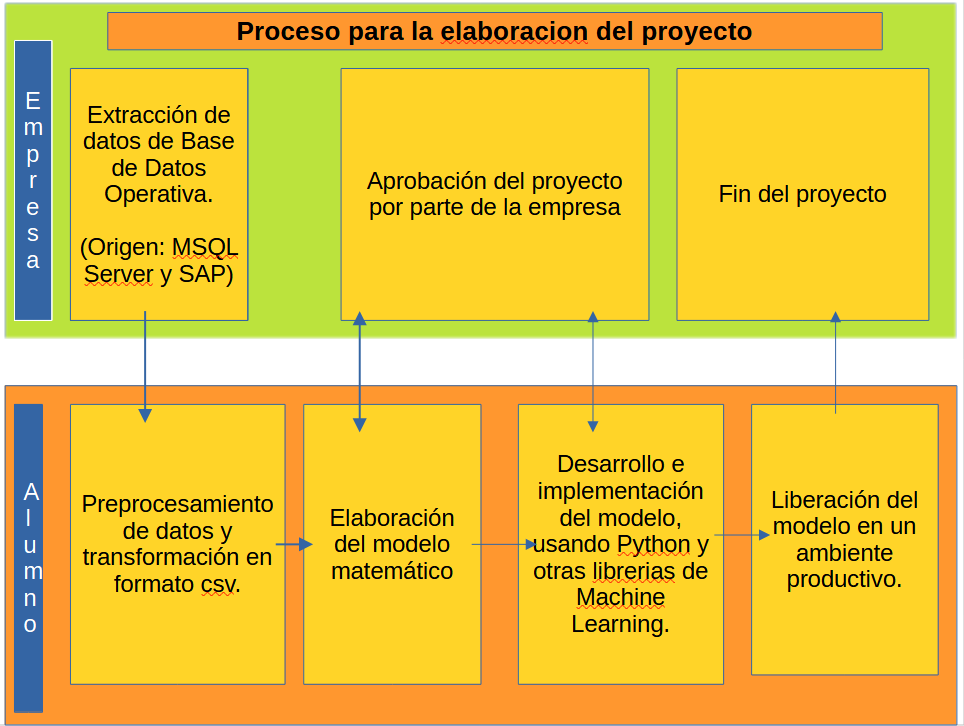
\includegraphics[width=12cm, height=7cm ]{Imagenes/Proceso_Proyecto.PNG }
      \caption{Metodología}
      \label{fig:meto}
  \end{figure}

La metodología para la realización del proyecto se explica con la figura anterior 13.

\begin{itemize}
    \item La empresa proporciona la información con la que quiere que se desarrolle el modelo en formato Excel. \medskip
    \item Se recibe el archivo Excel y se realiza la limpieza y preprocesamiento de datos y se convierte a un formato de texto CSV , para usarlo como entrada por el algoritmo de aprendizaje . \medskip
    \item Se elabora el modelo y se interactúa con la empresa , hasta lograr un modelo este de acuerdo a sus necesidades. \medskip
    \item Una vez aprobado el modelo, se desarrolla el algoritmo usando el lenguaje de programación Python y otras librerías adicionales.\medskip
    \item El script o programa es evaluado por la empresa, la cual da su aprobación en cuanto a la funcionalidad requerida. \medskip
    \item Completado el anterior paso la empresa da una carta de satisfacción de su proyecto , con lo cual queda concluido el proyecto terminal. \medskip
    
\end{itemize}


 
\section{Limpieza del dataset}

\section{Componentes auxiliares}

\section{Motor de inferencia}
